\subsection{Introduction}


bla


\subsection{Methods}
In this replication, we focus on the rate models proposed in the original article.
The firing rate model was an extensions of the traditional Wilson-Cowan model \supercite{wilson1972excitatory} and represented
an iso-frequency unit of the auditory cortex. This iso-frequency unit consisted of one excitatory and two inhibitory populations.
Building on this unit a more complex three-unit rate models was developed, to investigate stimulus-specific adaptation, forward suppression,
tunig-curve adaptation and feedforward functional connectivity. 

\paragraph{Iso-Frequency Unit Model}

The iso-frequency unit model was based on the Wilson-Cowan model \supercite{wilson1972excitatory} but was modified to include two different types of
inihbitory interneurons. The two inhibitory population are meant to represent parvalbumin-psoitive (PV) and somatostatin (SST) cells. The single unit
model is given by 
\begin{equation}
 \tau_u \frac{du(t)}{dt} = -u(t) + f(w_{ee}u(t) - w_{ep}p(t)- w_{es}s(t) + qg(t)i(t)), 
\end{equation}
 
\begin{equation}
 \tau_p \frac{dp(t)}{dt} = -p(t) + f(w_{pe}u(t) - w_{pp}p(t)- w_{ps}s(t) + I_{Opt,PV}(t) + qg(t)i(t)),
\end{equation}
 
\begin{equation} 
 \tau_s \frac{ds(t)}{dt} = -s(t) + f(w_{se}u(t) - w_{sp}p(t)- w_{ss}s(t) + I_{Opt,SST}(t),
\end{equation}
with $u(t)$, $p(t)$, and $s(t)$ being the normalized firing rates (in $[0,1]$) of the pyramidal cell population, the PV population and the SST population,
respectively. Furthermore, $w_xy$ represents the strengths of connections from population $y$ to population $x$. The two terms $I_{Opt,PV}$ and 
$I_{Opt,SST}$ describe the  input current to cells due to optogenetic stimulation of the PV population and SST population, respectively.
$\tau_i, i \in {u,p,s}$ defines the time constants for the respective populaitons. The function $f$ is realised as a threshold linear function
given by

\begin{equation}
 f(x) = \left \{ \begin{tabular}{c}
                0  \hspace{2em} if x\leq 0\\
                rx \hspace{2em} if 0<x\leq 1/r\\
                1  \hspace{2em} if x> 1/r,
               \end{tabular}

\end{equation}
which coarsely approximates a sigmoid function. Furthermore, the function $f$ is thresholded by simply subtracting a constant $u_i$ from the input
$x$ (i.e. $f(x-u_i)$) which varied for the different populations. Lastly, afferent auditory input is fed into the unit is given by $qg(t)i(t)$, which
is subdivided into the 'raw' input $i(t)$ and a slow modulation $g(t)$ mimicking synaptic depression at thalamic synapses. The input function $i(t)$
is simply an instantaneous rise with amplitude $q$ and an exponential decay with a time constant of $\tau_q$. The synaptic depression $g(t)$ is 
governed by the following equation
\begin{equation}
\label{eq:input_depression}
 \frac{dg(t)}{dt} = \frac{g_0-g(t)}{\tau_{d_1}} - \frac{g(t)i(t)}{\tau_{d_2}}.
\end{equation}

The parameter values can be found in Table \ref{tab:params}

\textbf{ToDo: Add parameter values to the table.}

\begin{table}
\begin{center}
\caption{Overview of the model parameters}
 \begin{tabular}{lcc}
  \toprule
  a & b & c \\
  \midrule
  1 & 2& 3 \\
  \bottomrule
 \end{tabular}
\label{tab:params}
\end{center}
\end{table}



\paragraph{Three-Unit Model}

Building on the single unit a three-unit model was implemented, with each single unit representing a different input frequency, thus creating a
simple tonotopic layout that allowed to explore more complex auditory inputs. Intra-unit connectivity was as described before for the single-uni 
model. Inter-unit connectivity was restricted to immediate neighbours and included the following connection types: Exc to exc, exc to PV and 
SST to exc. Together, the activity of the three populations of each unit was governed by
\begin{equation}
  \tau_u \frac{du_i(t)}{dt} = -u_i(t) + f(w_{ee}u_i(t) - (w_{ep} - a(1-D_i(t)))p_i(t)- w_{es}s_i(t) + J_{1,i}(t)), 
\end{equation}
\begin{equation}
  \tau_p \frac{dp_i(t)}{dt} = -p_i(t) + f(w_{pe}u_i(t) - w_{pp}p_i(t)- w_{ps}s_i(t) + I_{Opt,PV}(t) + J_{2,i}(t)), 
\end{equation}
\begin{equation}
  \tau_s \frac{ds_i(t)}{dt} = -s_i(t) + f(w_{se}u_i(t) - w_{sp}p_i(t)- w_{ss}s_i(t) + I_{Opt,SST}(t) + J_{3,i}(t)), 
\end{equation}
with
\begin{equation}
 J_{1,i}(t) =  \left \{ \begin{tabular}{c}
                $-F_i(t)s_2(t) + qI_i(t) + w_{ee}^*u_2(t)$  \hspace{10em} if $i=1,3 $\\
                $-F_s(t)(s_1(t)+ s_3(t)) + qI_2(t) + \frac{w_{ee}^*(u_1(t) + u_3(t))}{2} $ \hspace{2em} if $i=2$
               \end{tabular}

\end{equation}
and
\begin{equation}
 J_{2,i}(t) =  \left \{ \begin{tabular}{c}
                $qI_i(t) + w_{pe}^*u_2(t)$  \hspace{10em} if $i=1,3 $\\
                $qI_2(t) + \frac{w_{pe}^*(u_1(t) + u_3(t))}{2} $ \hspace{2em} if $i=2$
               \end{tabular}
\end{equation}
and
\begin{equation}
 J_{3,i}(t) =  \left \{ \begin{tabular}{c}
                $qI_i(t) + w_{se}^*u_2(t)$  \hspace{10em} if $i=1,3 $\\
                $qI_2(t) + \frac{w_{se}^*(u_1(t) + u_3(t))}{2} $ \hspace{2em} if $i=2$.
               \end{tabular}
\end{equation}
Here, $I_i(t)$ is described by
\begin{equation}
 I_k(t) = g_k(t)i_k(t)+g_2(t)i_2(t)\alpha \hspace{5em} \textnormal{for} \hspace{1em} k=1,3
\end{equation}
and
\begin{equation}
 I_2(t) = (g_1(t)i_1(t) + g_3(t)i_3(t))\alpha + g_2(t)i_2(t).
\end{equation}
Here, $i_k(t)$ represents thalamic inputs to each of the three units. Taken together, the description of the three-unit model is the same than 
for the single-unit model, except for the addition of lateral inter-unit connectivity and short-term synaptic dynamics. Short-term facilitation 
is modelled by $F_i(t)$ and increases from 0 to positive values whereas depression is modelled by $D_i(t)$, whic decreases from 1 towards 0. 
Facilitating synapses were added to Exc to SST inputs and depressing terms to PV to Exc synapses (see \supercite{beierlein2003two}). The facilitating
term $F_j(t)$ obeys
\begin{equation}
 \frac{dF_j(t)}{dt} = -\frac{F_j(t)}{\tau_{D_1}} + \frac{i_j(t)}{\tau_{D_2}},
\end{equation}
where $\tau_{D_1}$ and $\tau_{D_2}$ are again the depression time constants from the input functions of the single-unit model given in 
Equation \ref{eq:input_depression}. Analoguously, the depression term $D_j(t)$ follows
\begin{equation}
 \frac{dD_j(t)}{dt} = \frac{1-D_j(t)}{\tau_{D_1}} - \frac{D_j(t)i_j(t)}{\tau_{D_2}}.
\end{equation}
The choices for the parameters can again be found in Table \ref{tab:params} and were based on experimental studies \supercite{tsodyks1997paradoxical,
abbott1997synaptic,wehr2005synaptic}. 

Park and Geffen note that, when matching model behaviour to experimental findings, two distinct parameter sets emerged and a unified rate model 
description required a paradigm-dependent baseline inhibition, which reflected high thalamic activity (corresponding to weak baseline inhibition)
versus low thalamic activity (corresponding to strong baseline inhibition). This was implemented using another variable $\bar{F}$ governed by
\begin{equation}
  \frac{d\bar{F}(t)}{dt} = \frac{\bar{F}^2(t)}{\tau_{F_1}} - \frac{\bar{I}(t)}{\tau_{F_2}}.
\end{equation}

\textbf{ToDo: Add paragraph on the variable $F$} 


\subsection{Reimplementation}
The iso-frequency unit model and the three-unit model were both implemented in Python and integrated into the neurolib framework 
\supercite{cakan2019neurolib}.


\subsection{Reproduction of experiments}

\textbf{ToDo: Describe results}



\begin{figure}
\subfigure[original]{
 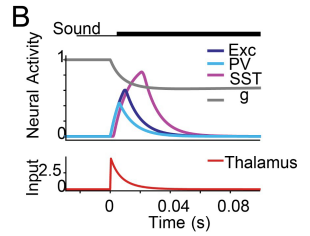
\includegraphics[width=\textwidth]{Figures/Original_Paper/Fig1B}}
\subfigure[replication]{
 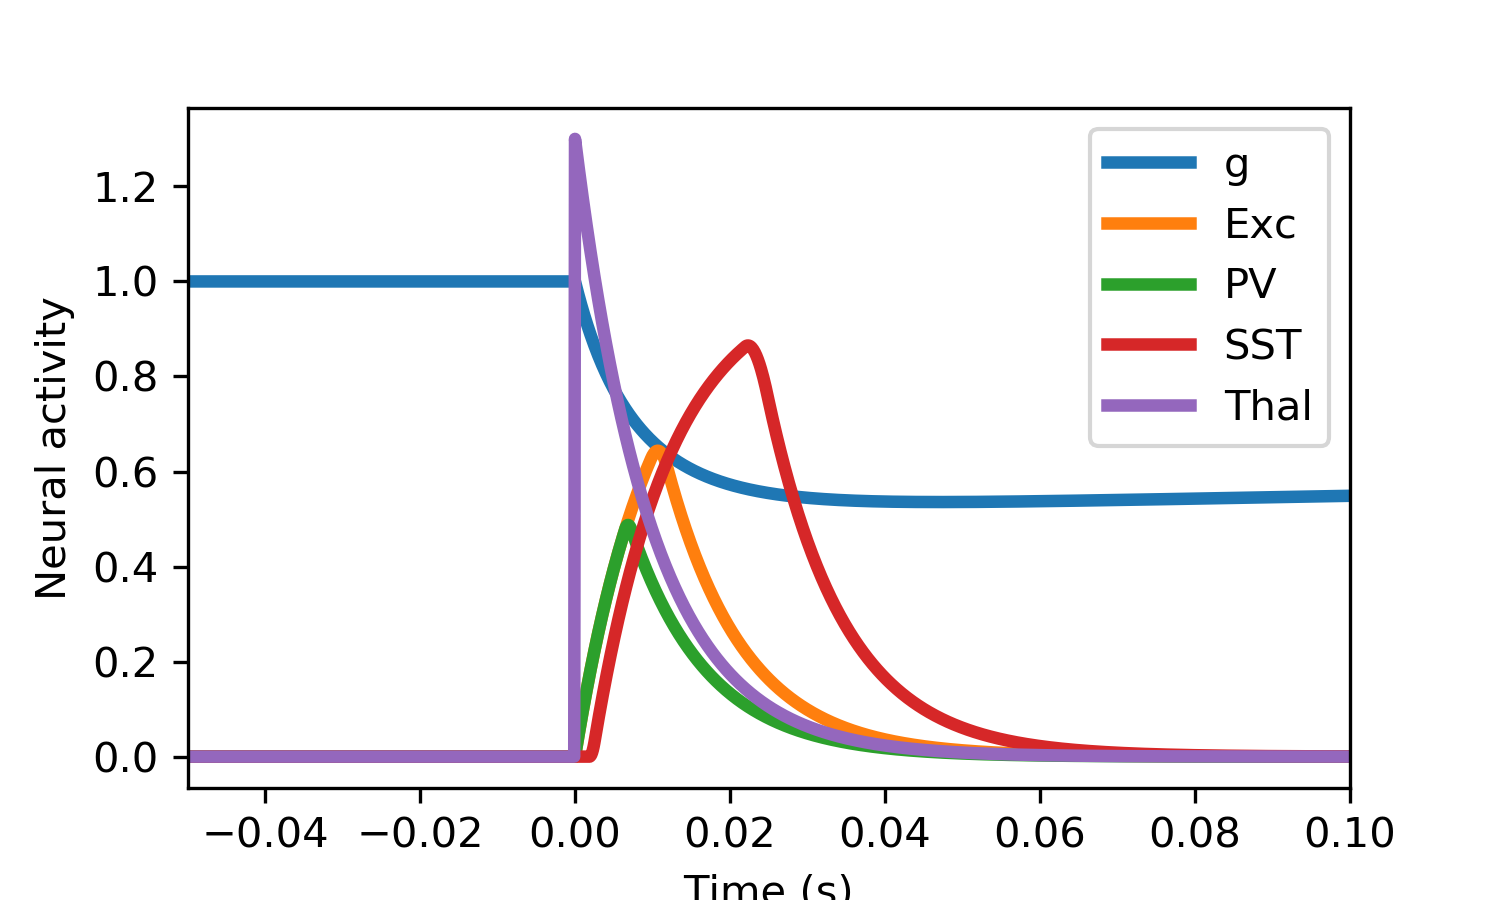
\includegraphics[width=\textwidth]{Figures/New_15_12_20/Fig1B}}
 \caption{Replicates Figure 1B.}
\end{figure}


\begin{figure}
 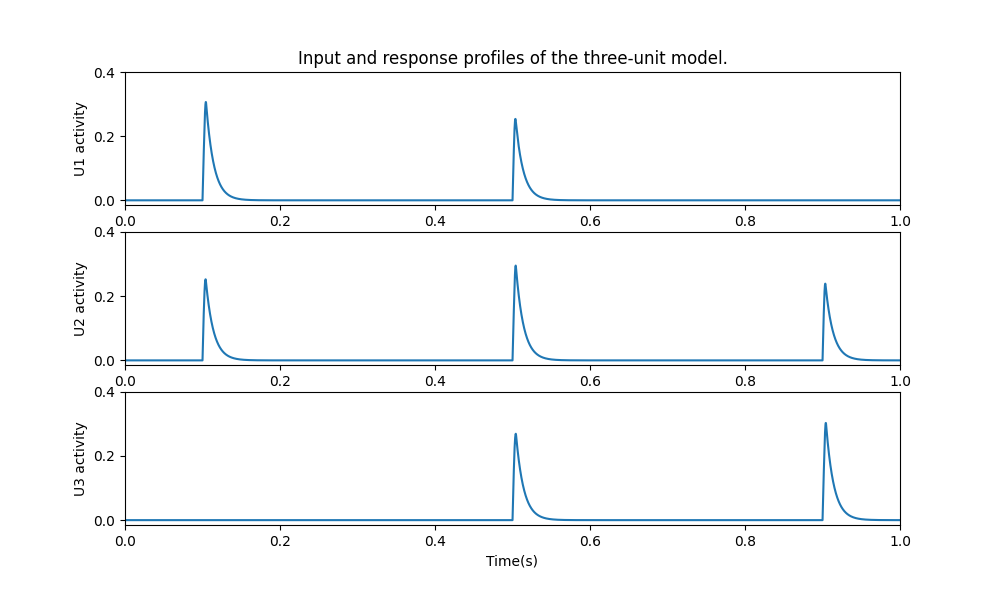
\includegraphics[width=\textwidth]{Figures/Fig2}
 \caption{ReFig2}
\end{figure}

\begin{figure}
 
 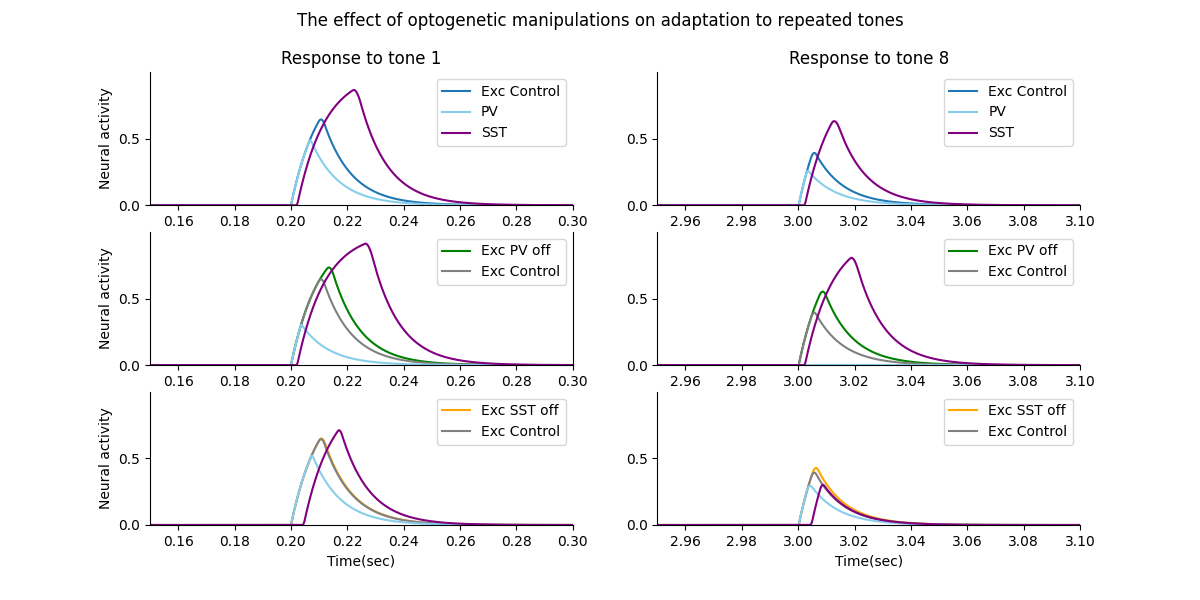
\includegraphics[width=\textwidth]{Figures/Fig3B}
 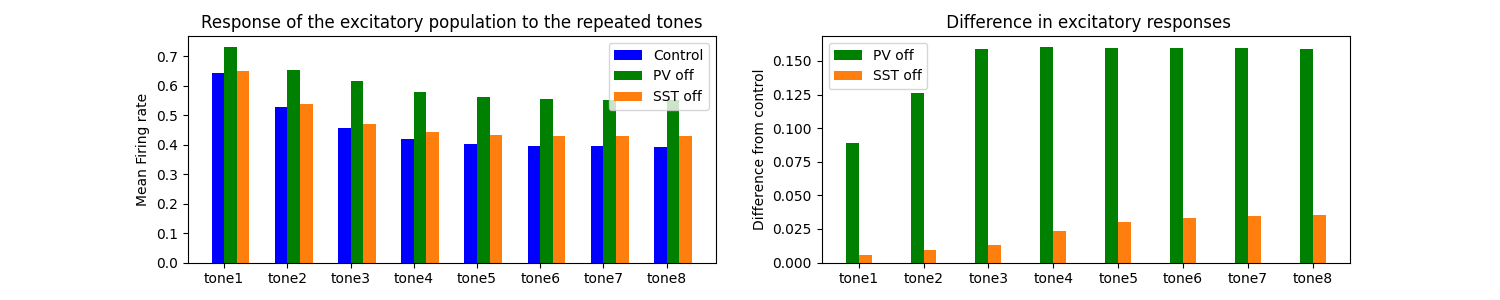
\includegraphics[width=\textwidth]{Figures/Fig3C}
 \caption{ReFig3}
\end{figure}

\begin{figure}
 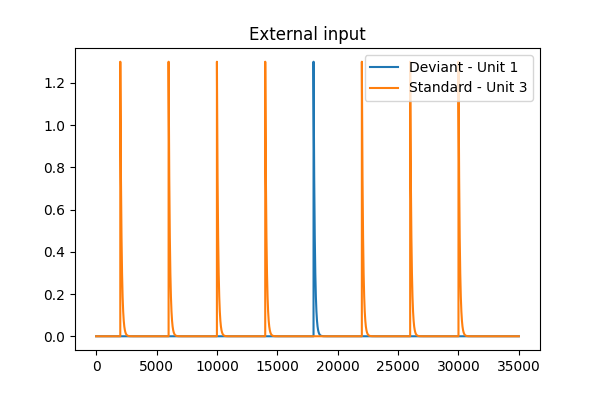
\includegraphics[width=\textwidth]{Figures/Fig4A}
 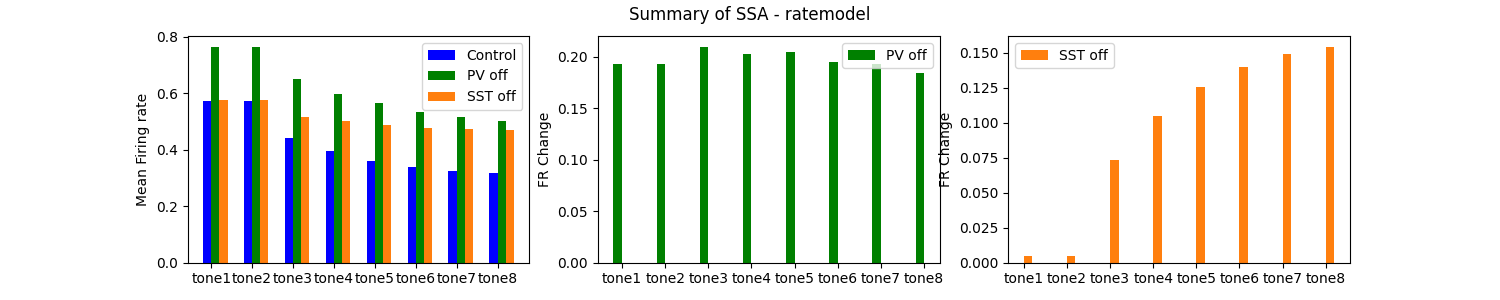
\includegraphics[width=\textwidth]{Figures/Fig4BDE}
 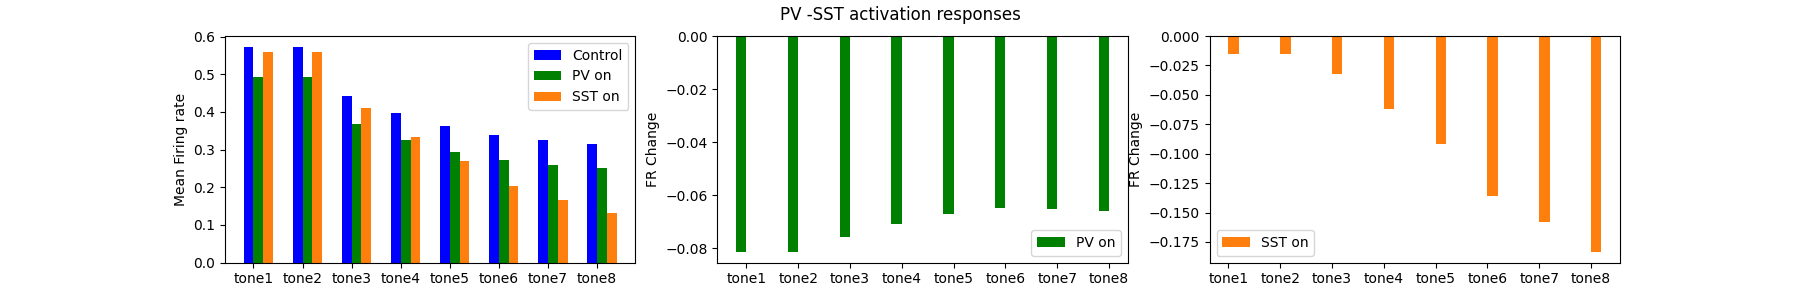
\includegraphics[width=\textwidth]{Figures/Fig4F}
 \caption{ReFig4}
\end{figure}

\begin{figure}
 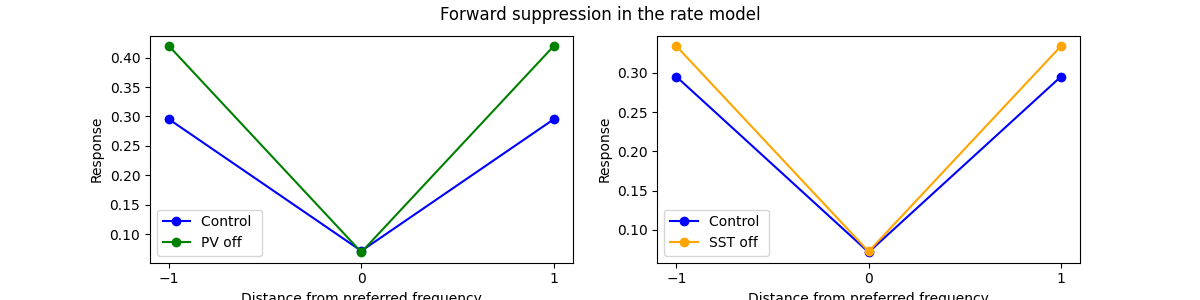
\includegraphics[width=\textwidth]{Figures/Fig6BC}
 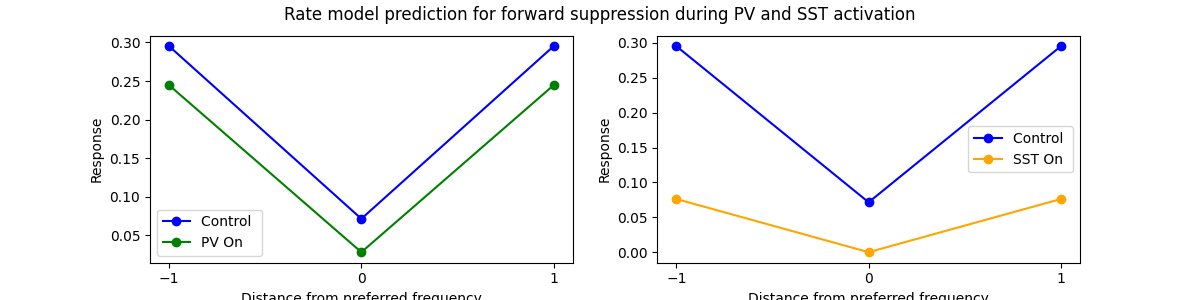
\includegraphics[width=\textwidth]{Figures/Fig6DE}
 \caption{ReFig6}
\end{figure}

\begin{figure}
 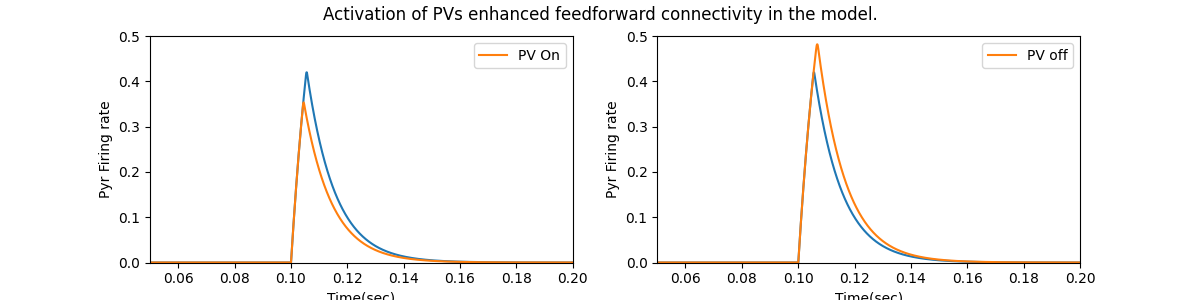
\includegraphics[width=\textwidth]{Figures/Fig8BD}
 \caption{ReFig8}
\end{figure}

\begin{figure}
 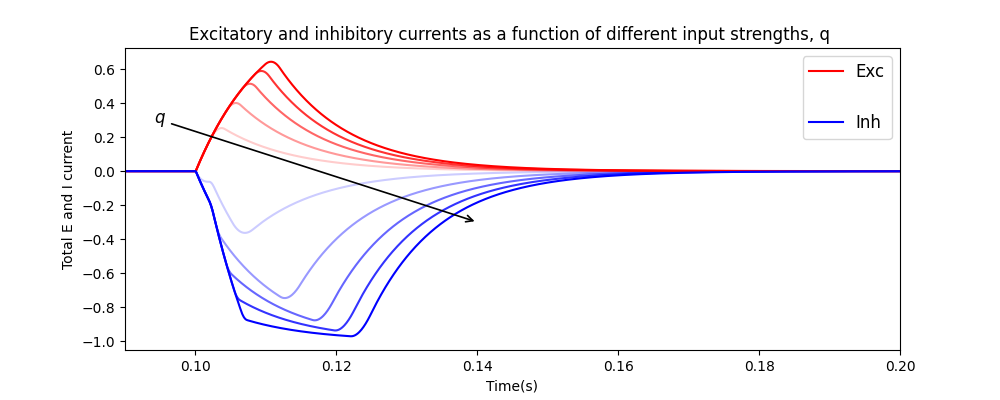
\includegraphics[width=\textwidth]{Figures/Fig9}
 \caption{ReFig9}
\end{figure}

 



\FloatBarrier
\subsection{Discussion}
bla

